\documentclass[t]{beamer}

% Load general definitions
% Preamble file - general definitions, package loading, etc.

%=================================
% Load packages
\usepackage{amssymb,amsmath}
\usepackage{graphicx}
\usepackage{url}
\usepackage{tikz}
\usetikzlibrary{mindmap,trees,arrows}
\usepackage{fancyvrb}
\usepackage[portuguese]{babel} 
\usepackage[utf8]{inputenc}
\usepackage{subfigure}
\usepackage{times}
\usepackage[T1]{fontenc}
\usepackage{cancel}
\usepackage{color}
\usepackage{listings}
\usepackage[document]{ragged2e}
\usepackage{physics}
\usepackage{amsmath}
\usepackage{tikz}
\usepackage{mathdots}
\usepackage{yhmath}
\usepackage{cancel}
\usepackage{color}
\usepackage{siunitx}
\usepackage{array}
\usepackage{multirow}
\usepackage{amssymb}
\usepackage{gensymb}
\usepackage{tabularx}
\usepackage{extarrows}
\usepackage{booktabs}
\usetikzlibrary{fadings}
\usetikzlibrary{patterns}
\usetikzlibrary{shadows.blur}
\usetikzlibrary{shapes}

%=================================
% Set mode
\mode<presentation>
{
	\usetheme{Madrid}
	\usecolortheme{structure}
	\useoutertheme{infolines}
	\setbeamercovered{invisible}
}

% Get rid of nav bar
\beamertemplatenavigationsymbolsempty

% Insert frame number at bottom of the page.
\usefoottemplate{\hfil\tiny{\color{black!90}\insertframenumber}} 

%=================================
% Define new commands

\newcommand\Real{{\mathbb{R}}}
%\newcommand{\vi}{\vspace{0.6\baselineskip}}
%\newcommand{\goodgap}{\hspace{\subfigtopskip}\hspace{\subfigbottomskip}}


% Equation environments
\newcommand{\beq}{\begin{equation}}
\newcommand{\eq}{\end{equation}}
\newcommand{\beqs}{\begin{equation*}}
\newcommand{\eqs}{\end{equation*}}
\newcommand{\beqn}{\begin{eqnarray}}
\newcommand{\eqn}{\end{eqnarray}}
% Bold variables
\newcommand{\mbf}[1]{\ensuremath{\mathbf{#1}}}
% Itemization
\newcommand{\bitem}{\begin{itemize}}
\newcommand{\eitem}{\end{itemize}}
\newcommand{\spitem}{\vskip 1em\item}
\newcommand{\bitems}{\begin{itemize}\item}
\newcommand{\benums}{\begin{enumerate}\item}
\newcommand{\eenum}{\end{enumerate}}
% color blocks
\newenvironment{colorblock}[2]{%
\setbeamercolor{block title}{#2}
\begin{block}{#1}}{\end{block}}
% Vertical spacing
\newcommand{\vone}{\vskip 1em}
\newcommand{\vhalf}{\vskip .5em}
% Frame environments
\newenvironment{ftst}[3][t]{%
\begin{frame}{environment=ftst,#1}
\frametitle{#2}
\framesubtitle{#3}}{\end{frame}}
\newenvironment{ftstf}[2]{
\begin{frame}[fragile,environment=ftstf]
\frametitle{#1}
\framesubtitle{#2}}{\end{frame}}
% colors
\definecolor{MyGray}{rgb}{0.5,0.5,0.5}
\definecolor{MyDBGray}{rgb}{0.1,0.1,0.4}
\definecolor{darkgreen}{rgb}{0,0.4,0}
\definecolor{black}{rgb}{0,0,0}
\def\defn#1{{\color{red} #1}}
% Footnote
\renewcommand{\thefootnote}{\alph{footnote}}
% Relaxed footnotes
\newcommand{\lfr}[1]{\let\thefootnote\relax\footnote{\tiny #1}}
% Verbatim environment - using FANCYVRB package
\DefineVerbatimEnvironment%
{rcode}{Verbatim}
{fontsize=\scriptsize}
% Verbatim environment - using LISTINGS package
%\lstnewenvironment{rcode} {\lstset{	language = R,
%									basicstyle = \scriptsize\ttfamily,
%									showspaces = false,
%									showstringspaces = false,
%									showtabs = false,
%									keywordstyle = \color{black}\bfseries,
%									commentstyle = \color{darkgreen},
%									numbers = none,
%									otherkeywords={	<-,
%													ggplot,
%													geom_boxplot,
%													facet_grid,
%													shapiro.test,
%													fligner.test,
%													glht,
%													with},
%									deletekeywords={data,
%													model,
%													residuals,
%													c,
%													axis,
%													default,
%													labels,
%													qq.text}}}%
%{}

% Specific definitions
\title[]{Banco de dados II}
\subtitle[]{O modelo Entidade-Relacionamento Estendido (EER)}
\author[]{Patrícia Lucas\\{\footnotesize }}
\institute{Bacharelado em Sistemas de Informação \\ IFNMG  - Campus Salinas}
\date{\scriptsize Salinas\\Julho 2021}

\begin{document}

% cover page
\setbeamertemplate{footline}{}
\begin{frame}

\begin{center}
\includegraphics[width=.15\textwidth]{}
\end{center}
  \titlepage
  \begin{tikzpicture}[remember picture,overlay]
  \node[anchor=south east,xshift=-5pt,yshift=5pt] at (current page.south east) {\tiny Versão 1.2021};
  \node[anchor=south west,yshift=0pt] at (current page.south west) {
\includegraphics[width=.25\textwidth]{Logos/salinas_horizontal_jpg.jpg}};
  \end{tikzpicture}  
\end{frame}

% Main slides

\begin{ftst}{Referência}{Modelo Entidade-Relacionamento Estendido}
\begin{figure}
    \centering
    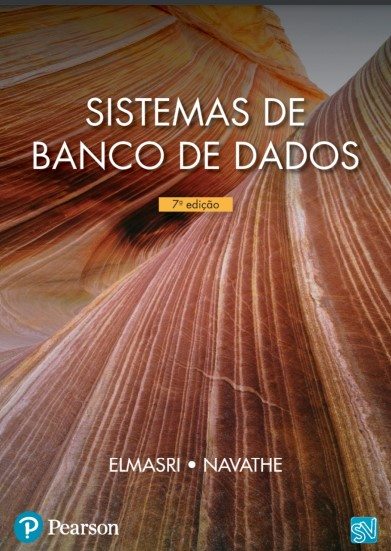
\includegraphics[scale=0.4]{Figuras/book.jpg}
\end{figure}
ELMASRI, R.; NAVATHE, S. B. Sistemas de Banco de Dados. 7. ed. São Paulo: Pearson Addison Wesley, 2019.
\end{ftst}

%==================================

\begin{ftst}{Subclasses, superclasses e herança}{Modelo Entidade-Relacionamento Estendido}
\small
\begin{itemize}
    \item Em muitos casos, uma entidade tem diversos subagrupamentos ou subtipos que são significativos e precisam ser representados explicitamente, por causa de seu significado para a aplicação de banco de dados.
    \item Exemplo: entidade FUNCIONÁRIO podem ser distinguidas ainda mais em SECRETARIA, ENGENHEIRO, GERENTE, TÉCNICO, FUNCIONARIO\_MENSAL e FUNCIONARIO\_HORISTA.
    \item O conjunto de entidades em cada um desses agrupamentos é um subconjunto das entidades que pertencem ao conjunto de entidades FUNCIONÁRIO, significando que cada entidade que é membro de um desses subagrupamentos também é um funcionário.
    \item Chamamos cada um desses subagrupamentos de \textbf{subclasse} do tipo de entidade FUNCIONÁRIO, e o tipo de entidade FUNCIONÁRIO é chamado de \textbf{superclasse} para cada uma dessas subclasses.
\end{itemize}
\end{ftst}

%==================================

\begin{ftst}{Subclasses, superclasses e herança}{Modelo Entidade-Relacionamento Estendido}
\begin{itemize}
    \item Notação:
\end{itemize}

\begin{figure}
    \centering
    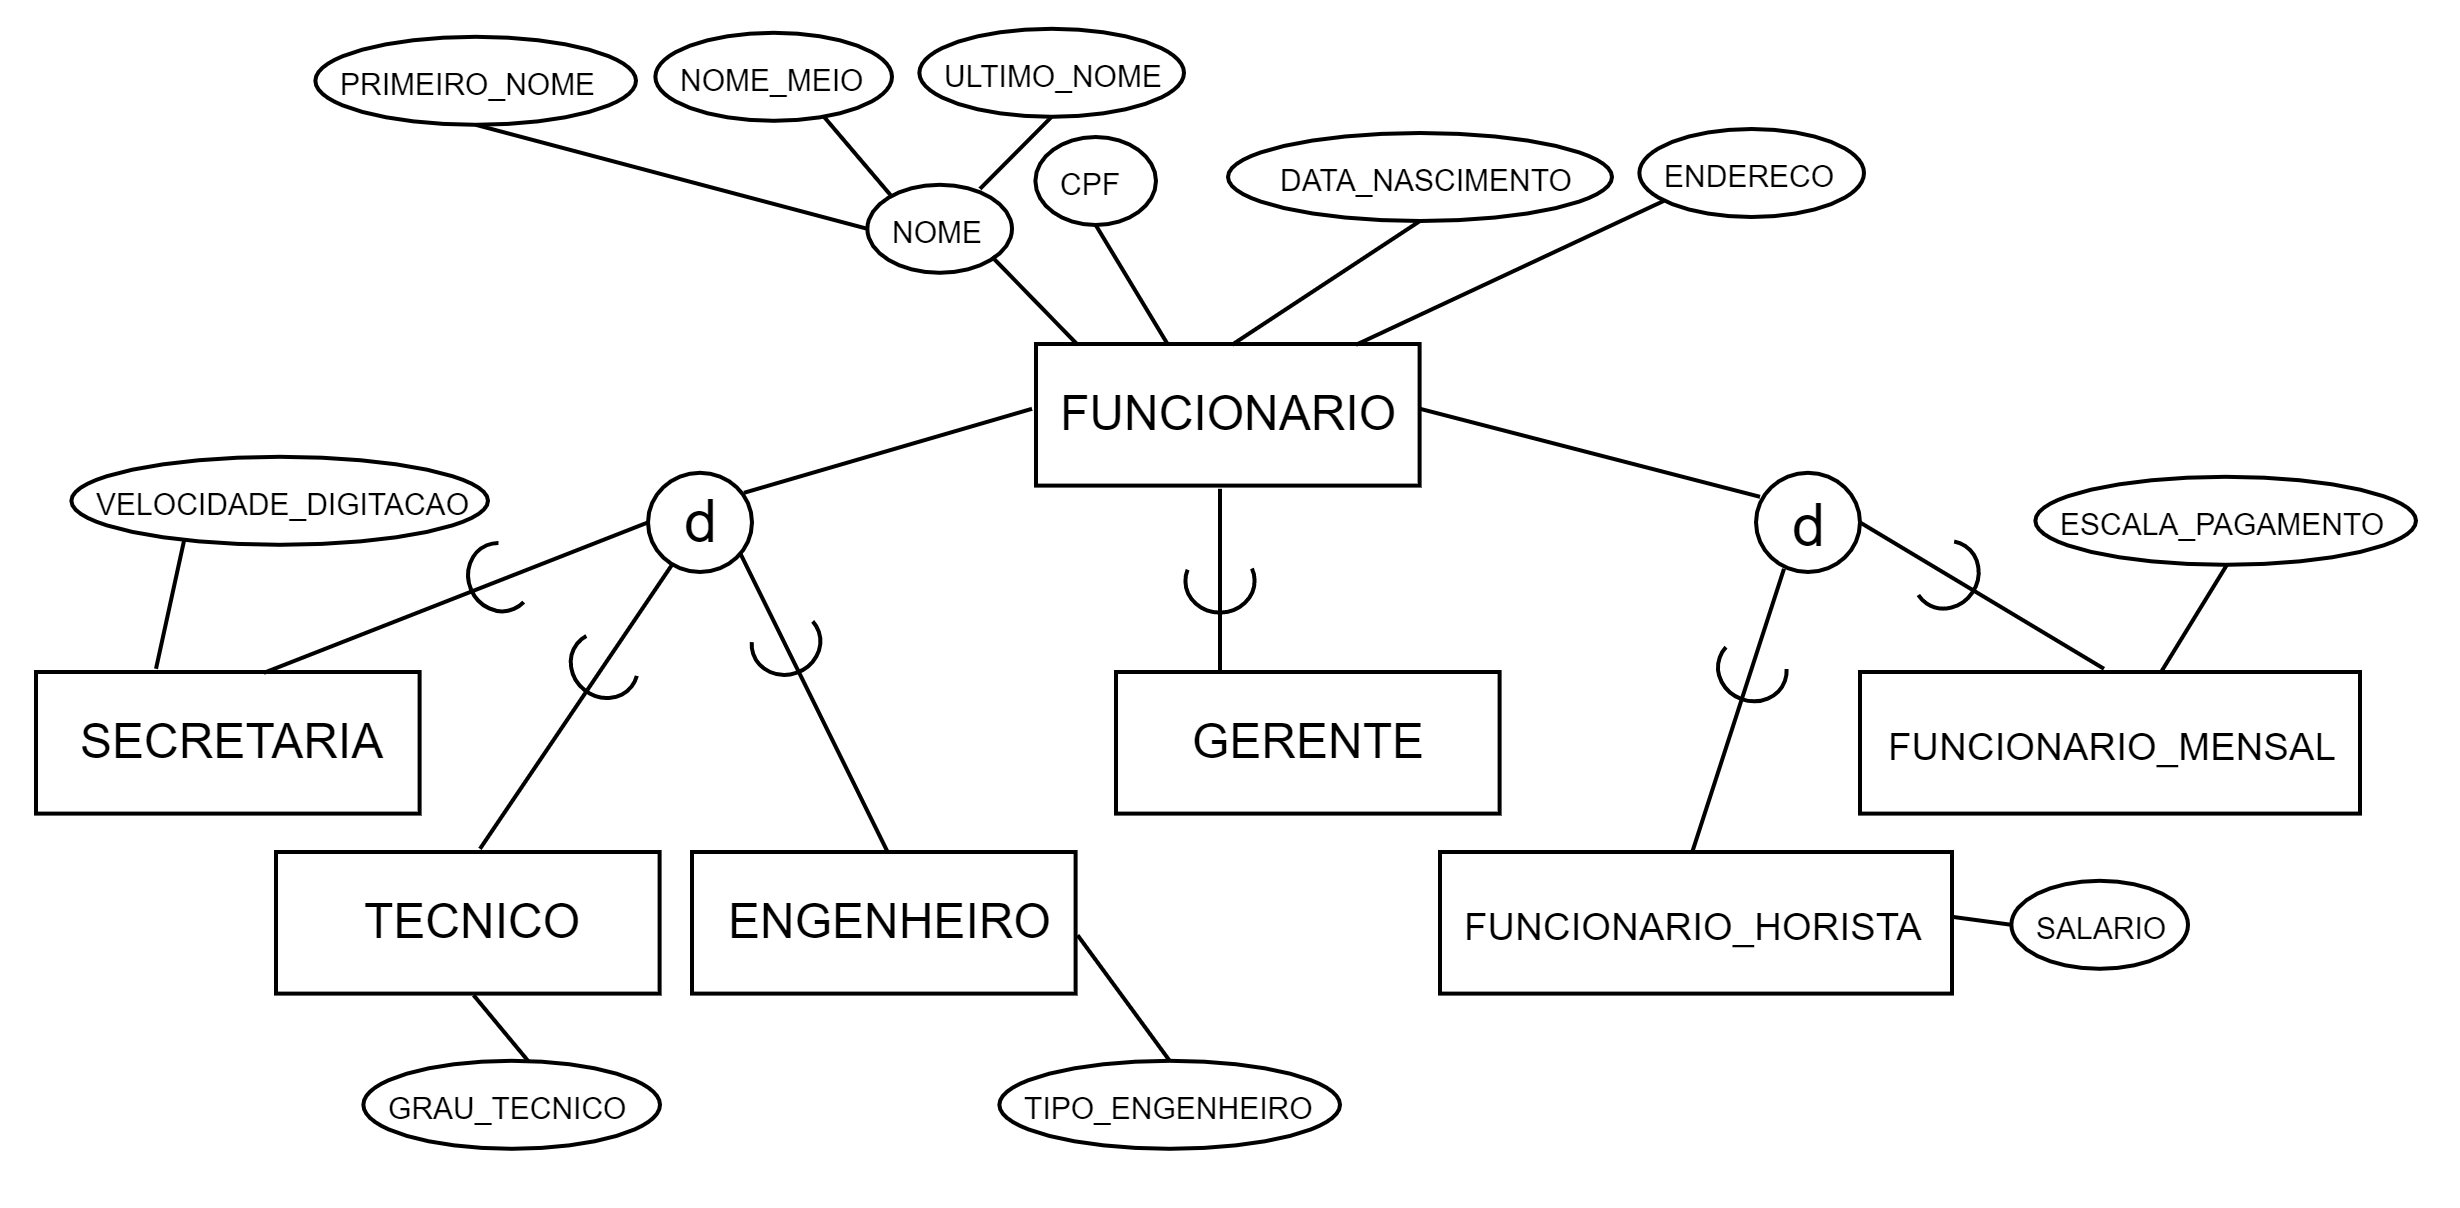
\includegraphics[scale=0.13]{Figuras/02_1.png}
\end{figure}

\end{ftst}

%==================================

\begin{ftst}{Subclasses, superclasses e herança}{Modelo Entidade-Relacionamento Estendido}
\small
\begin{itemize}
    \item Chamamos o relacionamento entre uma superclasse e qualquer uma de suas subclasses de \textbf{relacionamento superclasse/subclasse}.
    \item Uma entidade não pode existir no banco de dados simplesmente por ser um membro de uma subclasse, ela também precisa ser um membro da superclasse.
    \item Essa entidade pode ser incluída opcionalmente como um membro de qualquer número de subclasses. Exemplo: um funcionário assalariado que também é um engenheiro pertence às duas subclasses, ENGENHEIRO e FUNCIONARIO\_MENSAL.
    \item Não é necessário que toda entidade em uma superclasse seja um membro de alguma subclasse.
\end{itemize}
\end{ftst}

%==================================

\begin{ftst}{Subclasses, superclasses e herança}{Modelo Entidade-Relacionamento Estendido}
\small
\begin{itemize}
    \item Um conceito importante associado às subclasses é o de herança.
    \item Lembre-se de que o tipo de uma entidade é definido pelos atributos que ela possui e os tipos de relacionamento de que participa. Como uma entidade na subclasse representa a mesma entidade do mundo real da superclasse, ela deve possuir valores para seus atributos específicos, bem como valores de seus atributos como um membro da superclasse. 
    \item Dizemos que uma entidade que é um membro de uma subclasse \textbf{herda} todos os atributos da entidade como um membro da superclasse.
    \item A entidade também herda todos os relacionamentos de que a superclasse participa.
\end{itemize}
\end{ftst}

%==================================

\begin{ftst}{Especialização}{Modelo Entidade-Relacionamento Estendido}
\small
\begin{itemize}
    \item Especialização é o processo de definir um conjunto de subclasses de uma entidade.
    \item O conjunto de subclasses que forma uma especialização é definido com base em alguma característica distinta das entidades na superclasse.
    \item Podemos ter várias especializações da mesma entidade com base em características distintas. 
    \item Exemplo: o conjunto de subclasses {SECRETARIA, ENGENHEIRO, TÉCNICO} é uma especialização da superclasse FUNCIONÁRIO, que distingue as entidades do funcionário com base no tipo de cargo de cada um. Já a especialização baseada no método de pagamento da entidade FUNCIONÁRIO pode gerar o conjunto de subclasses {FUNCIONARIO\_MENSAL, FUNCIONARIO\_HORISTA}.
\end{itemize}
\end{ftst}

%==================================

\begin{ftst}{Especialização}{Modelo Entidade-Relacionamento Estendido}
\small
\begin{itemize}
    \item Os atributos das subclasses são chamados \textbf{atributos específicos}.
    \item Uma subclasse pode participar de tipos de \textbf{relacionamento específicos}.
    \item Um relacionamento de superclasse/subclasse assemelha-se a um relacionamento 1:1 no nível de instância.
    \item Motivos principais para incluir relacionamentos de classe/subclasse e especializações:
    \begin{itemize}
        \item Quando certos atributos podem se aplicar a algumas, mas não a todas as entidades do tipo superclasse.
        \item Quando alguns tipos de relacionamento podem participar apenas de entidades que são membros da subclasse.
    \end{itemize}
\end{itemize}
\end{ftst}

%==================================

\begin{ftst}{Generalização}{Modelo Entidade-Relacionamento Estendido}
\begin{itemize}
    \item Usamos o termo generalização para nos referir ao processo de definição de uma entidade generalizada com base nas entidade dadas.
    \item O processo de generalização pode ser visto como o inverso do processo de especialização.
    \item Exemplo: podemos ver CARRO e CAMINHAO como uma especialização de VEICULO, ou VEICULO como uma generalização de CARRO e CAMINHAO.
\end{itemize}
\end{ftst}

%==================================

\begin{ftst}{Restrições sobre especialização e generalização}{Modelo Entidade-Relacionamento Estendido}
\small
\begin{itemize}
    \item Restrição de \textbf{disjunção}:
    \begin{itemize}
        \item Especifica que as subclasses da especialização devem ser disjuntas, ou seja, uma entidade pode ser um
membro de no máximo uma das subclasses da especialização.
        \item Notação \textbf{"d"}.
        \item Exemplo: um FUNCIONARIO ou é FUNCIONARIO\_MENSAL ou é FUNCIONARIO\_HORISTA.
    \end{itemize}
\end{itemize}
\begin{figure}
    \centering
    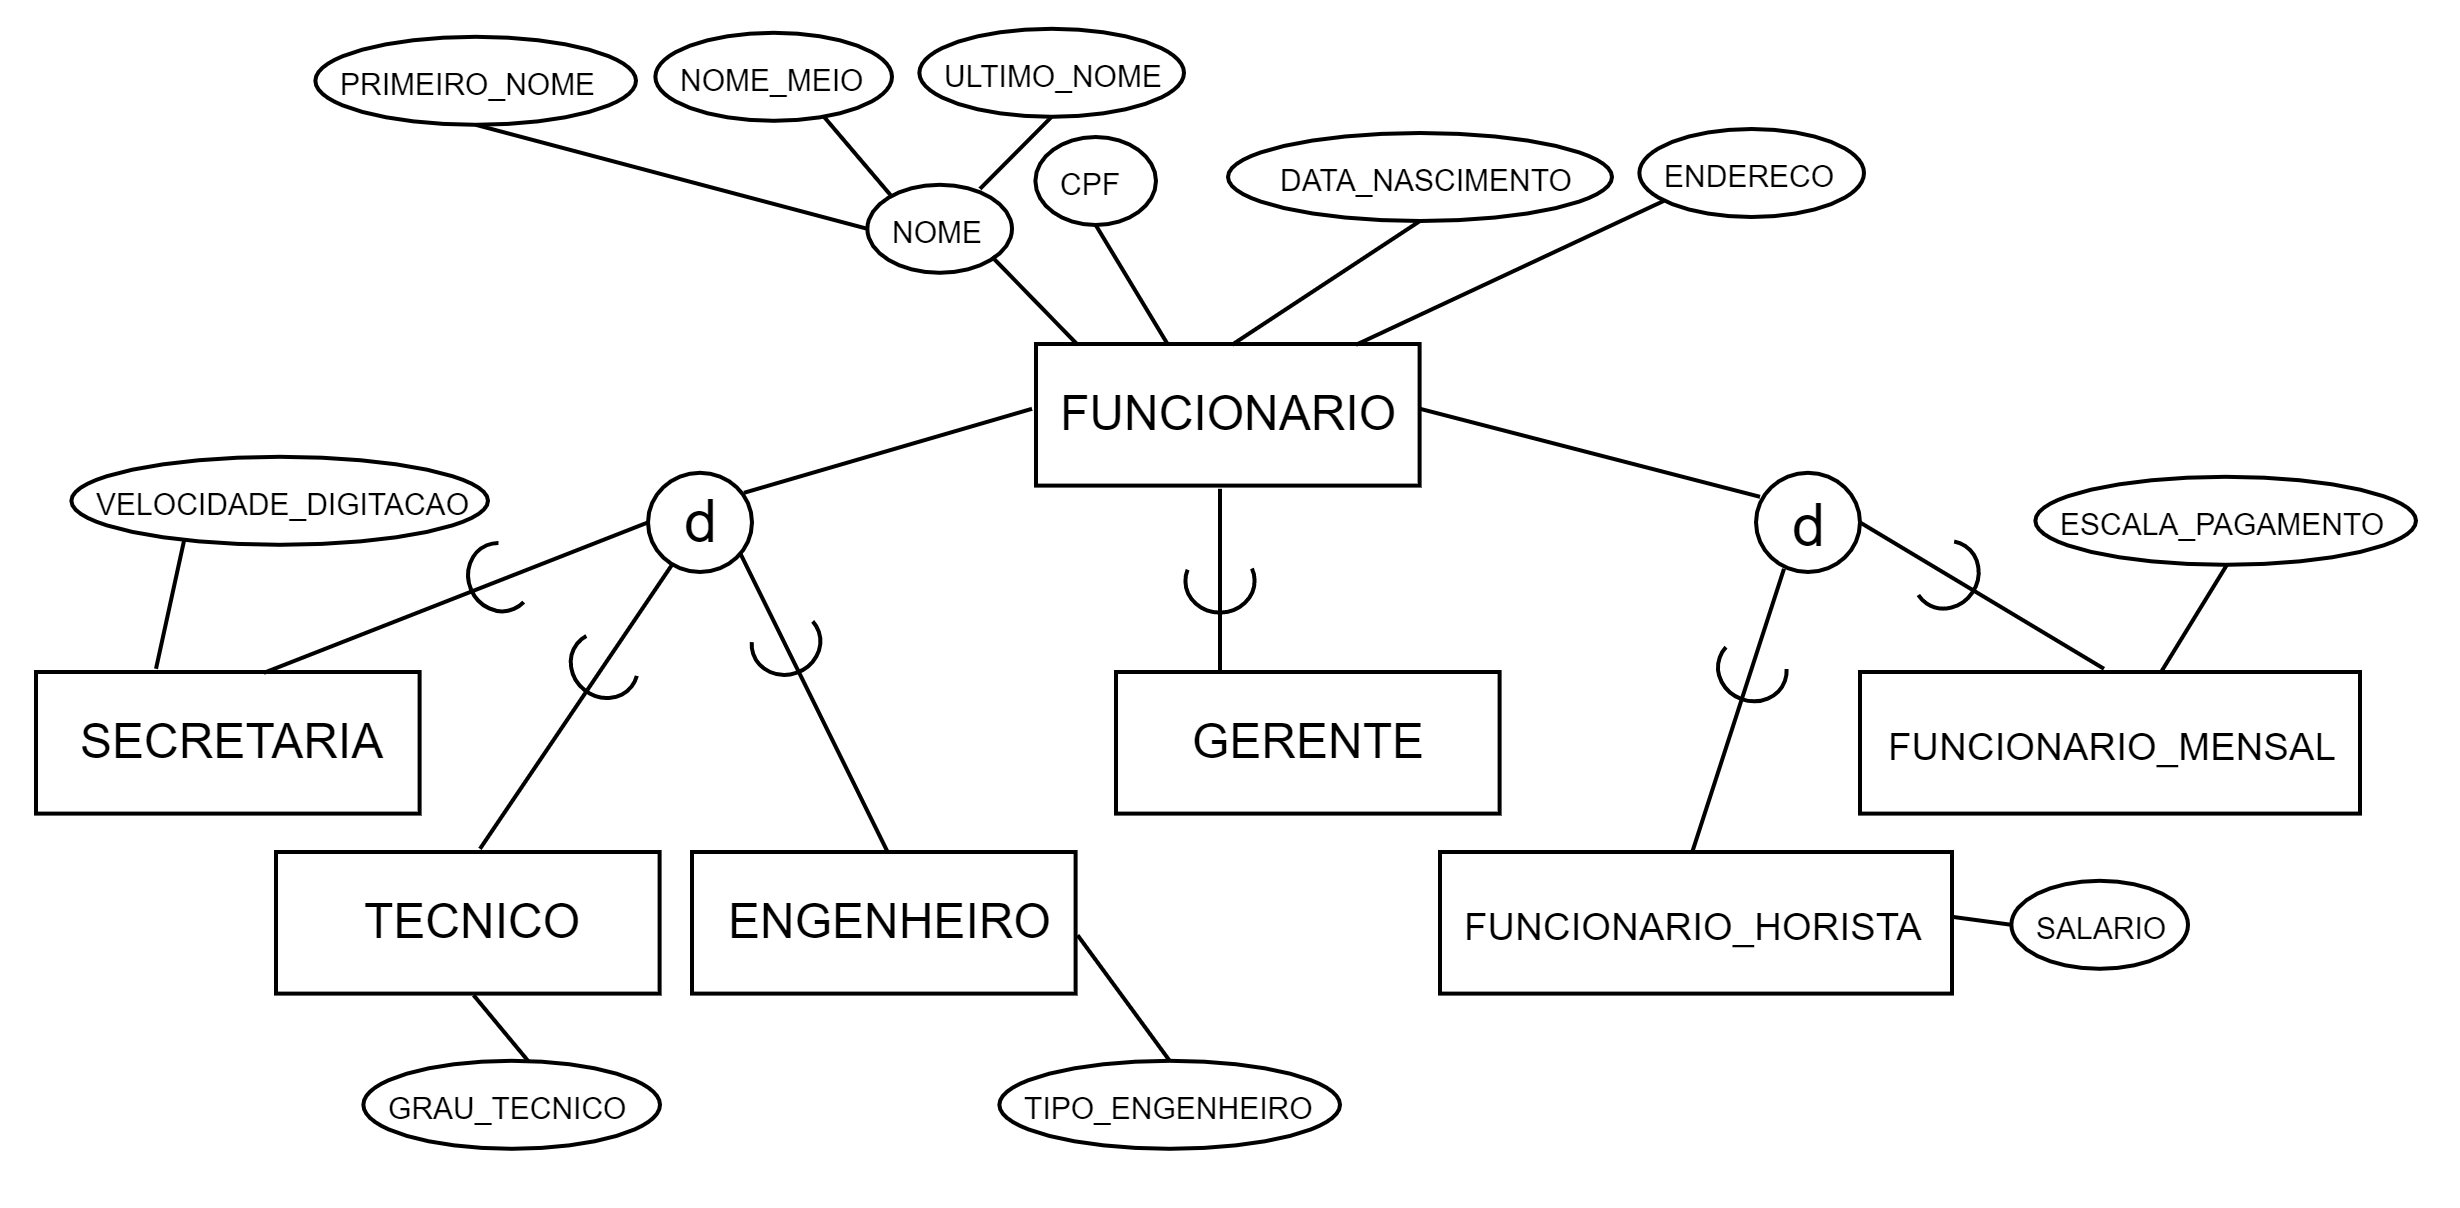
\includegraphics[scale=0.10]{Figuras/02_1.png}
\end{figure}

\end{ftst}

%==================================

\begin{ftst}{Restrições sobre especialização e generalização}{Modelo Entidade-Relacionamento Estendido}
\small
\begin{itemize}
    \item Se as subclasses não forem restringidas a serem disjuntas, seus conjuntos de entidades podem ser \textbf{sobrepostos (overlapping)}, ou seja, a mesma entidade pode ser um membro de mais de uma subclasse da especialização.
    \item Notação \textbf{"o"}.
    \item Exemplo: Uma PECA pode ser FABRICADA e COMPRADA.
\end{itemize}
\begin{figure}
    \centering
    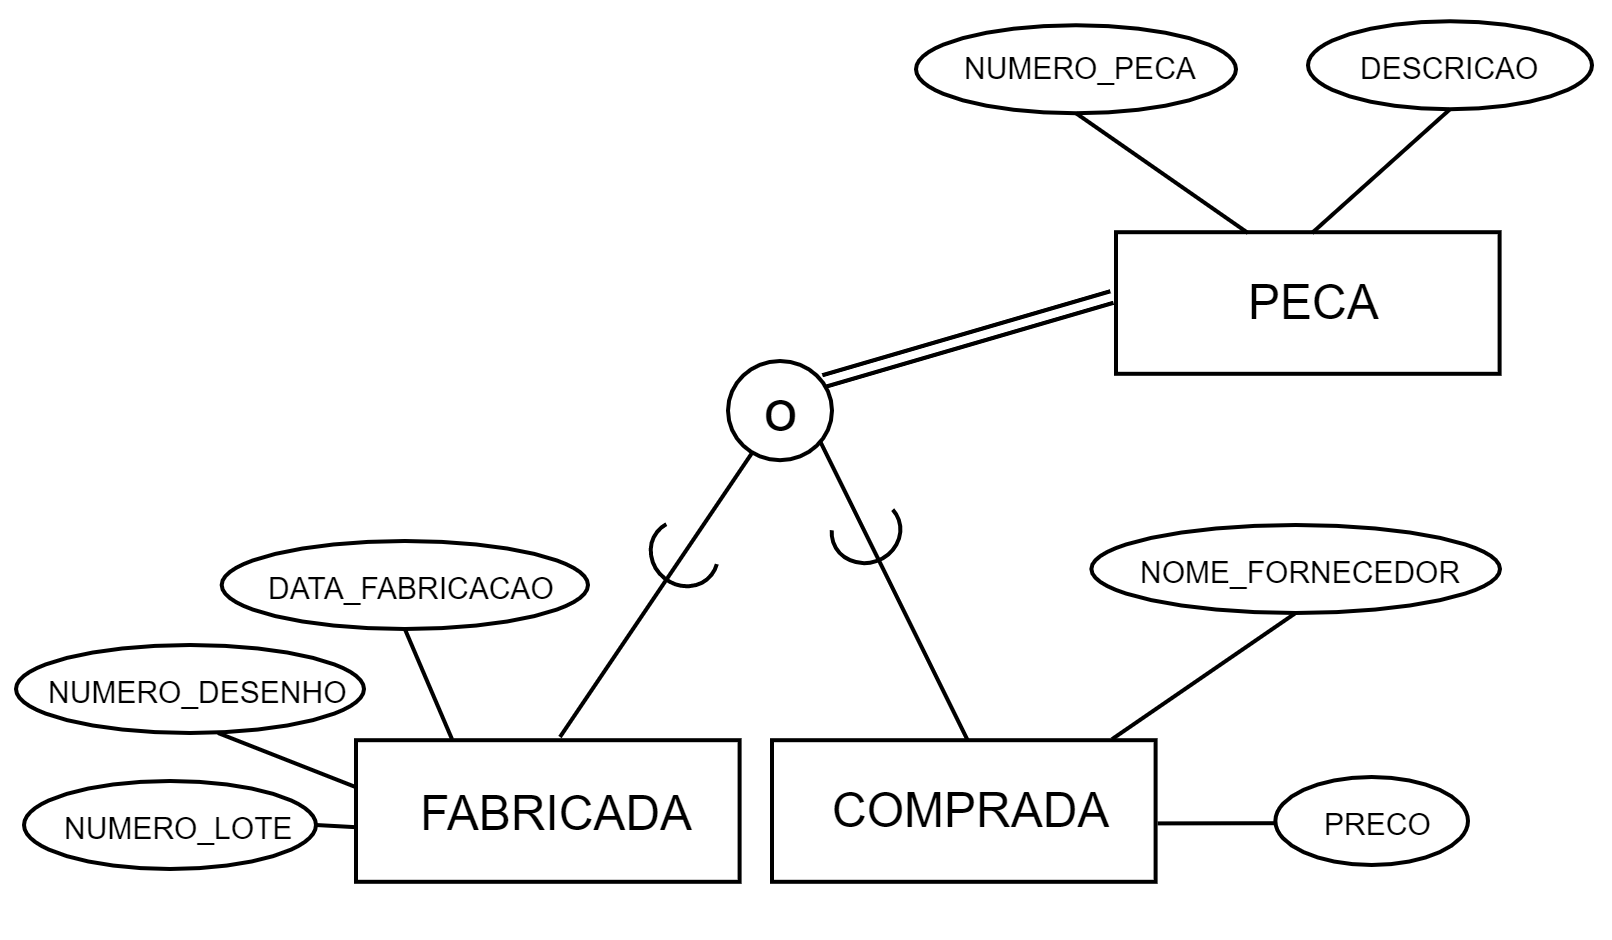
\includegraphics[scale=0.13]{Figuras/02_2.png}
\end{figure}

\end{ftst}

%==================================

\begin{ftst}{Restrições sobre especialização e generalização}{Modelo Entidade-Relacionamento Estendido}
\small
\begin{itemize}
    \item Restrição de \textbf{completude ou totalidade}:
    \begin{itemize}
        \item \textbf{Total: }especifica que toda entidade na superclasse precisa ser um membro de pelo menos uma subclasse na especialização.
        \item Exemplo: toda PECA deve ser especializada.
        \item Notação: linha dupla.
    \end{itemize}
\end{itemize}
\begin{figure}
    \centering
    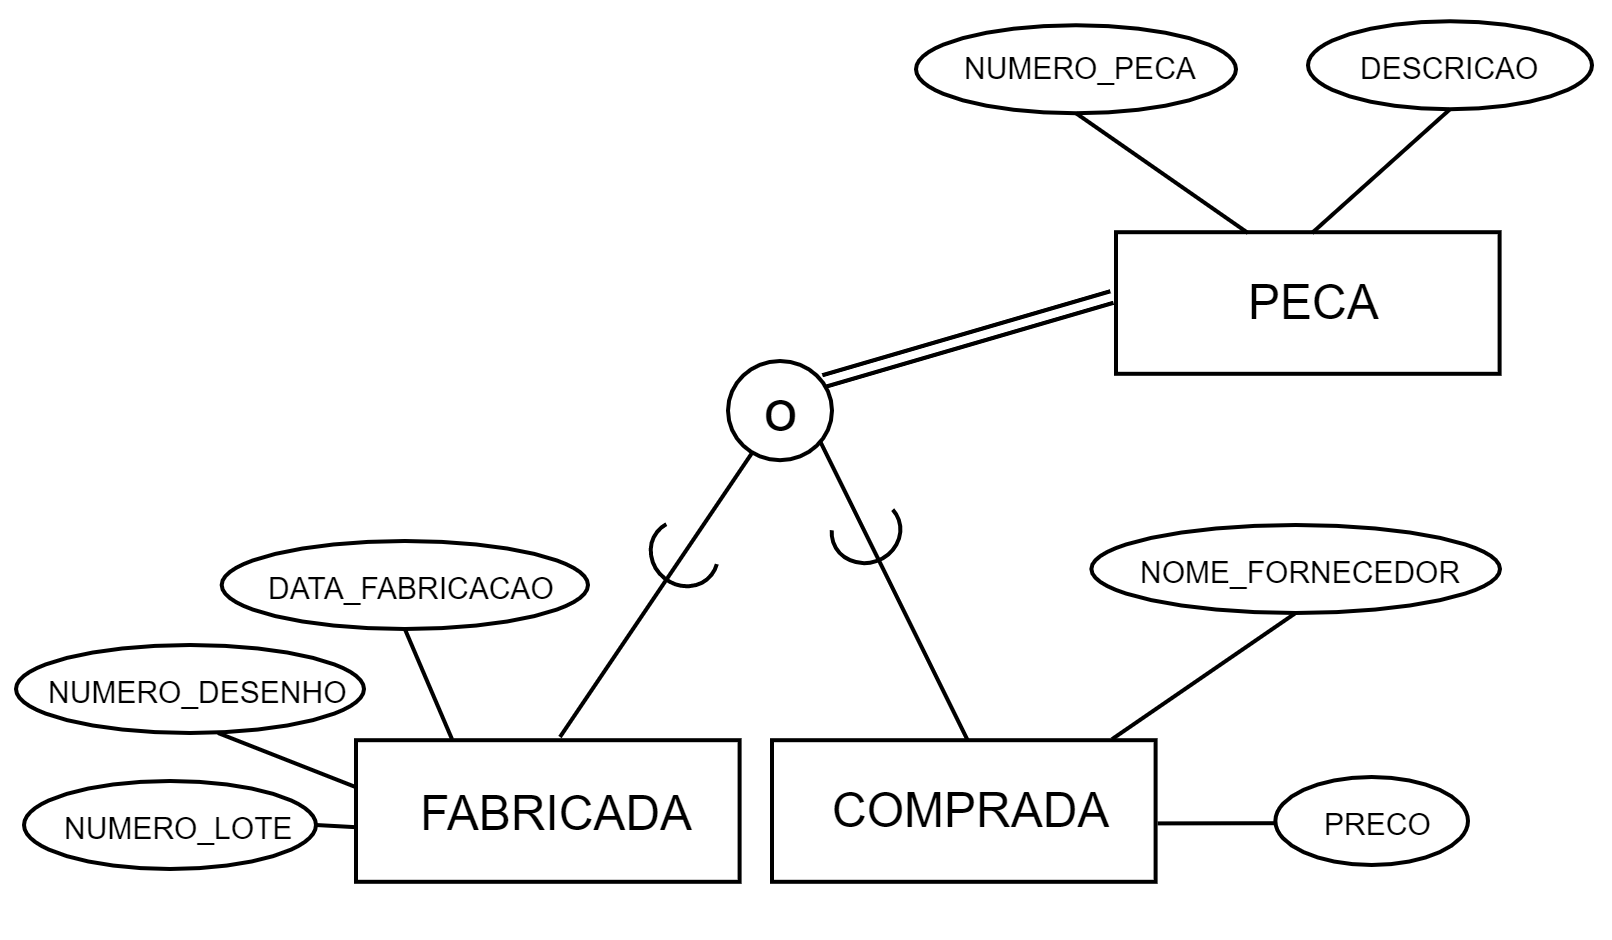
\includegraphics[scale=0.13]{Figuras/02_2.png}
\end{figure}

\end{ftst}

%==================================

\begin{ftst}{Restrições sobre especialização e generalização}{Modelo Entidade-Relacionamento Estendido}
\small
\begin{itemize}
    \item Restrição de \textbf{completude ou totalidade}:
    \begin{itemize}
        \item \textbf{Parcial:} permite que uma entidade não pertença a qualquer uma das subclasses.
        \item Exemplo: FUNCIONARIO não pertencerem a nenhuma das subclasses {SECRETARIA, ENGENHEIRO, TECNICO}.
        \item Notação: linha simples.
    \end{itemize}
\end{itemize}
\begin{figure}
    \centering
    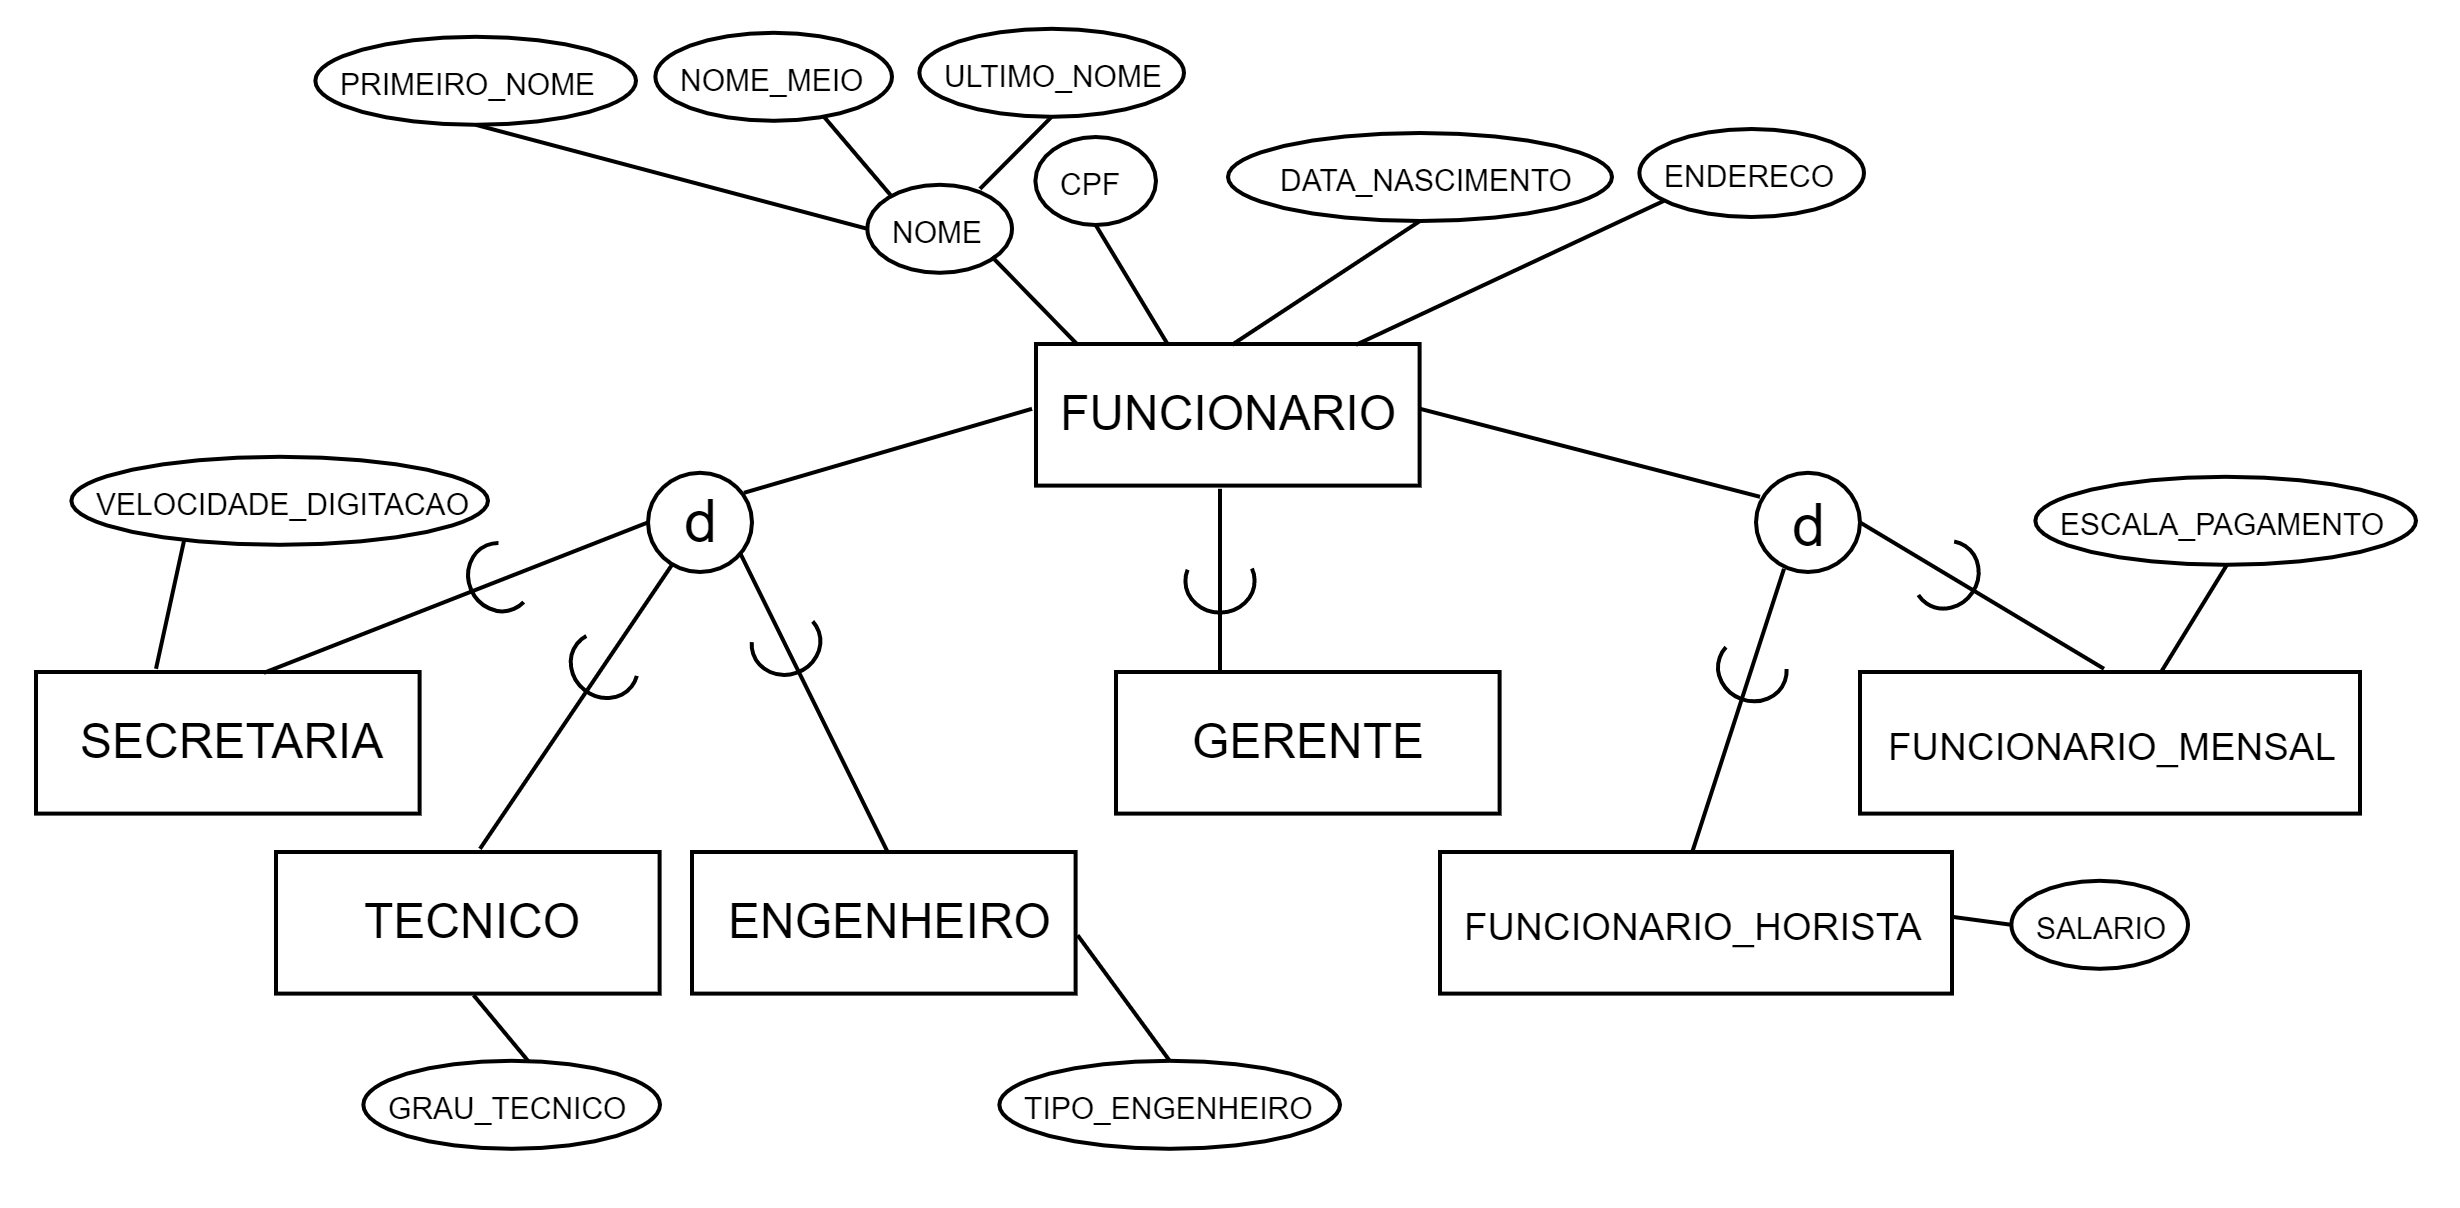
\includegraphics[scale=0.1]{Figuras/02_1.png}
\end{figure}

\end{ftst}

%==================================

\begin{ftst}{Restrições sobre especialização e generalização}{Modelo Entidade-Relacionamento Estendido}

\begin{itemize}
    \item as restrições de disjunção e completude são independentes, logo, temos quatro restrições possíveis na especialização:
    \begin{itemize}
        \item Disjunção, total.
        \item Disjunção, parcial.
        \item Sobreposição, total.
        \item Sobreposição, parcial.
    \end{itemize}
\end{itemize}
\end{ftst}

%==================================

\begin{ftst}{Hierarquias e reticulado da especialização e generalização}{Modelo Entidade-Relacionamento Estendido}

\begin{itemize}
    \item Uma subclasse pode ter mais subclasses especificadas nela, formando uma hierarquia ou um reticulado de especializações. 
    \item Exemplo: ENGENHEIRO é uma subclasse de FUNCIONÁRIO e também uma superclasse de GERENTE-ENGENHEIRO.
\end{itemize}
\begin{figure}
    \centering
    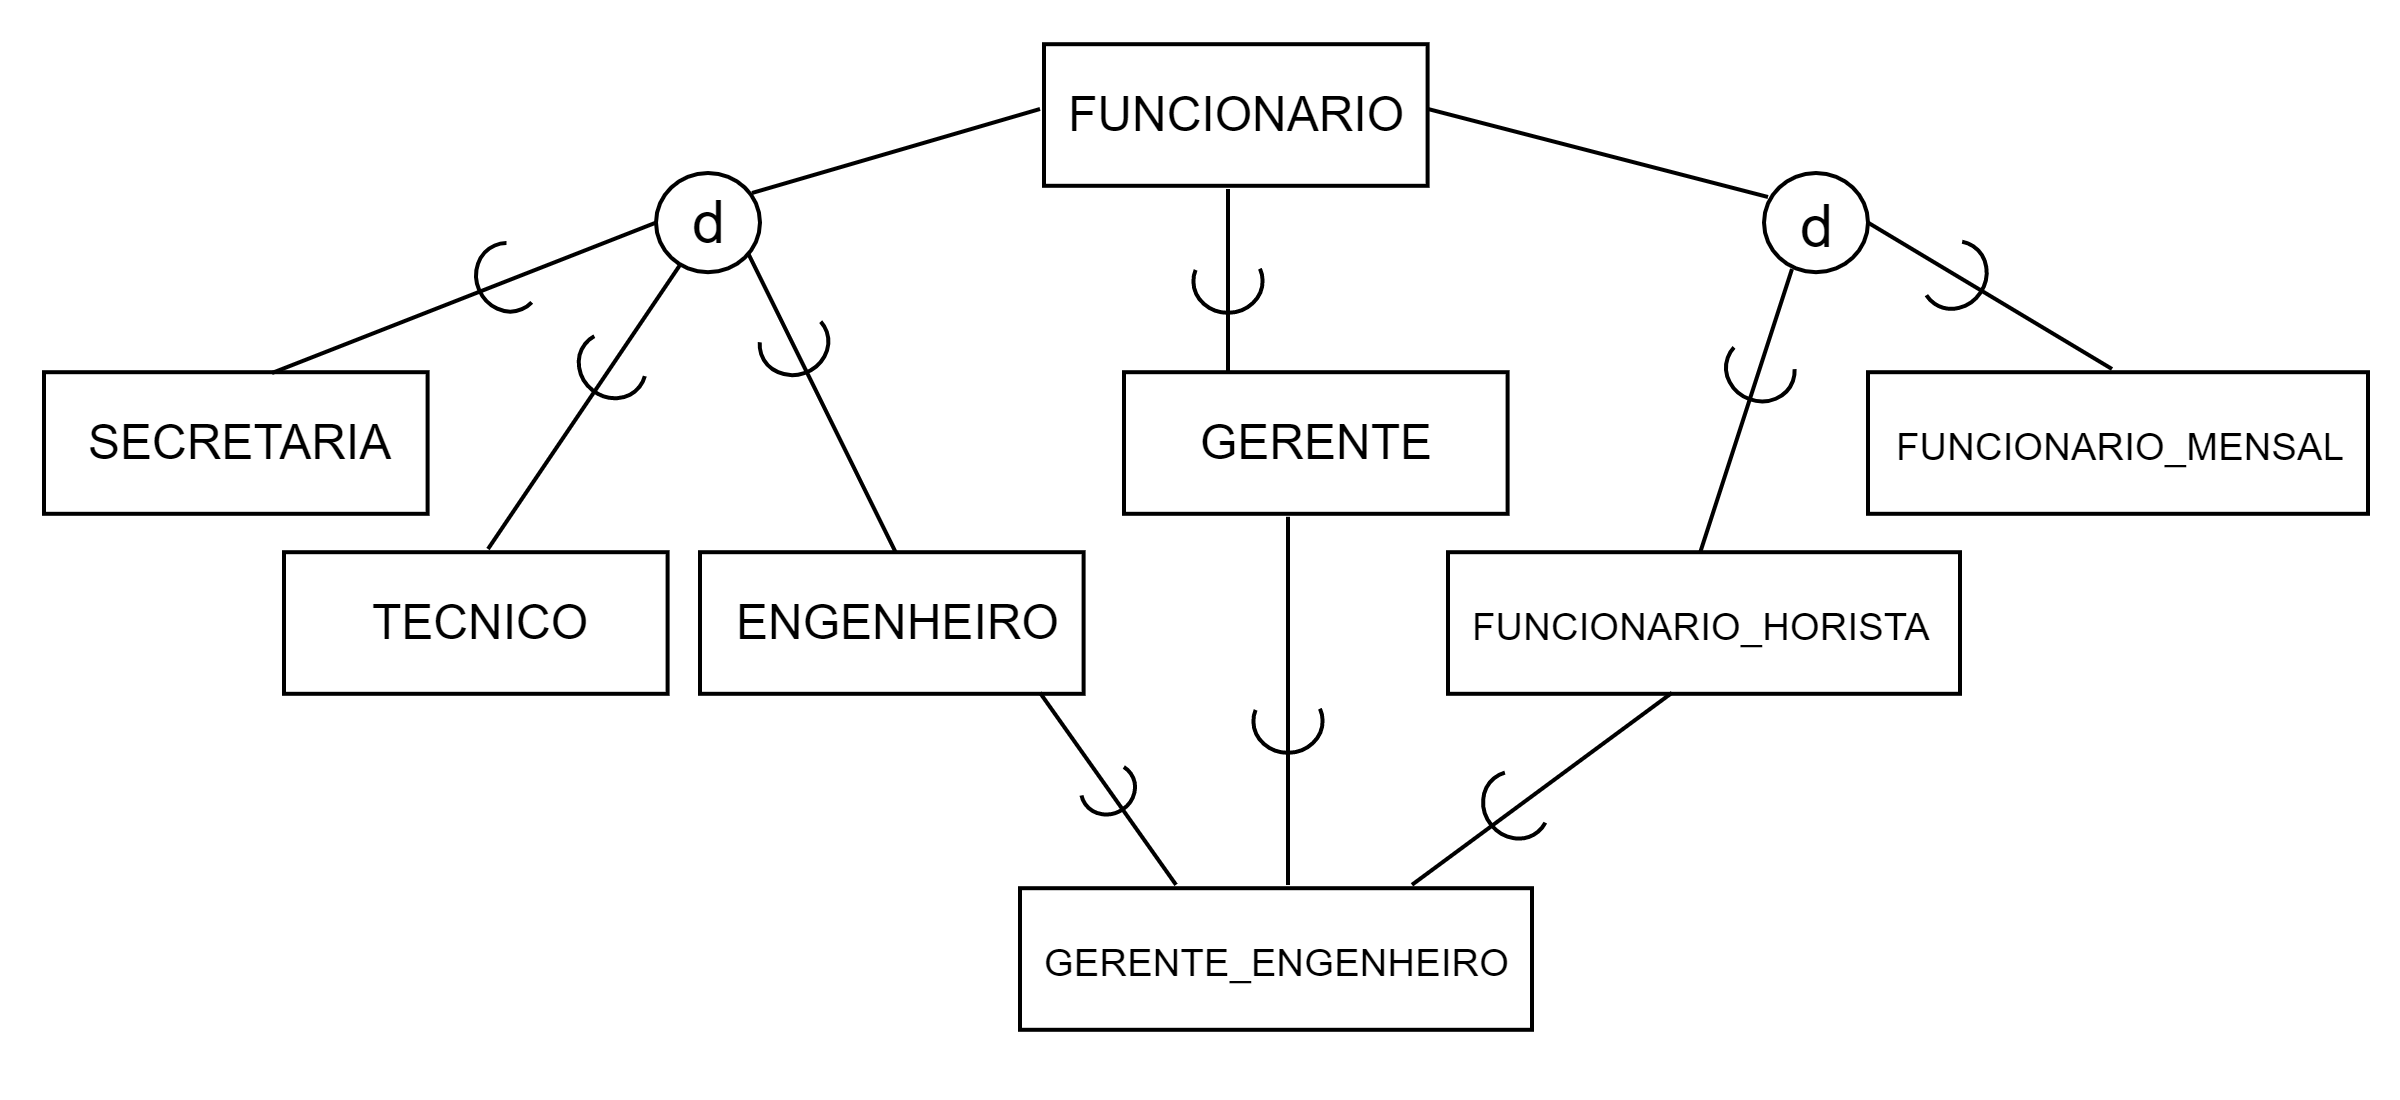
\includegraphics[scale=0.13]{Figuras/02_03.png}
\end{figure}
\end{ftst}

%==================================

\begin{ftst}{Hierarquias e reticulado da especialização e generalização}{Modelo Entidade-Relacionamento Estendido}

\begin{itemize}
    \item \textbf{Hierarquia:} tem a restrição de que cada subclasse participa como uma subclasse em apenas um relacionamento de classe/subclasse.
    \item \textbf{Reticulado:} uma subclasse pode ser uma subclasse em mais de um relacionamento de classe/subclasse.
    \item Em um reticulado ou hierarquia de especialização, uma subclasse herda os atributos não só de sua superclasse direta, mas também de todas as suas superclasses predecessoras, até chegar à raiz da hierarquia ou reticulado, se for preciso.
\end{itemize}
\end{ftst}

%==================================

\begin{ftst}{Modelagem dos tipos UNIÃO usando categorias}{Modelo Entidade-Relacionamento Estendido}
\footnotesize
\begin{itemize}
    \item As vezes é necessário representar uma coleção de entidades a partir de diferentes tipos de entidade.
    \item Neste caso, a subclasse representará uma coleção de entidades que é um subconjunto da UNIÃO de entidades de tipos distintos. \item Essa subclasse é chamada de \textbf{tipo de união} ou \textbf{categoria}.
    \item Exemplo: Uma categoria PROPRIETÁRIO, que é uma subclasse da UNIÃO dos três conjuntos de entidades de EMPRESA, BANCO e PESSOA.
    \item Notação:
\end{itemize}
\begin{figure}
    \centering
    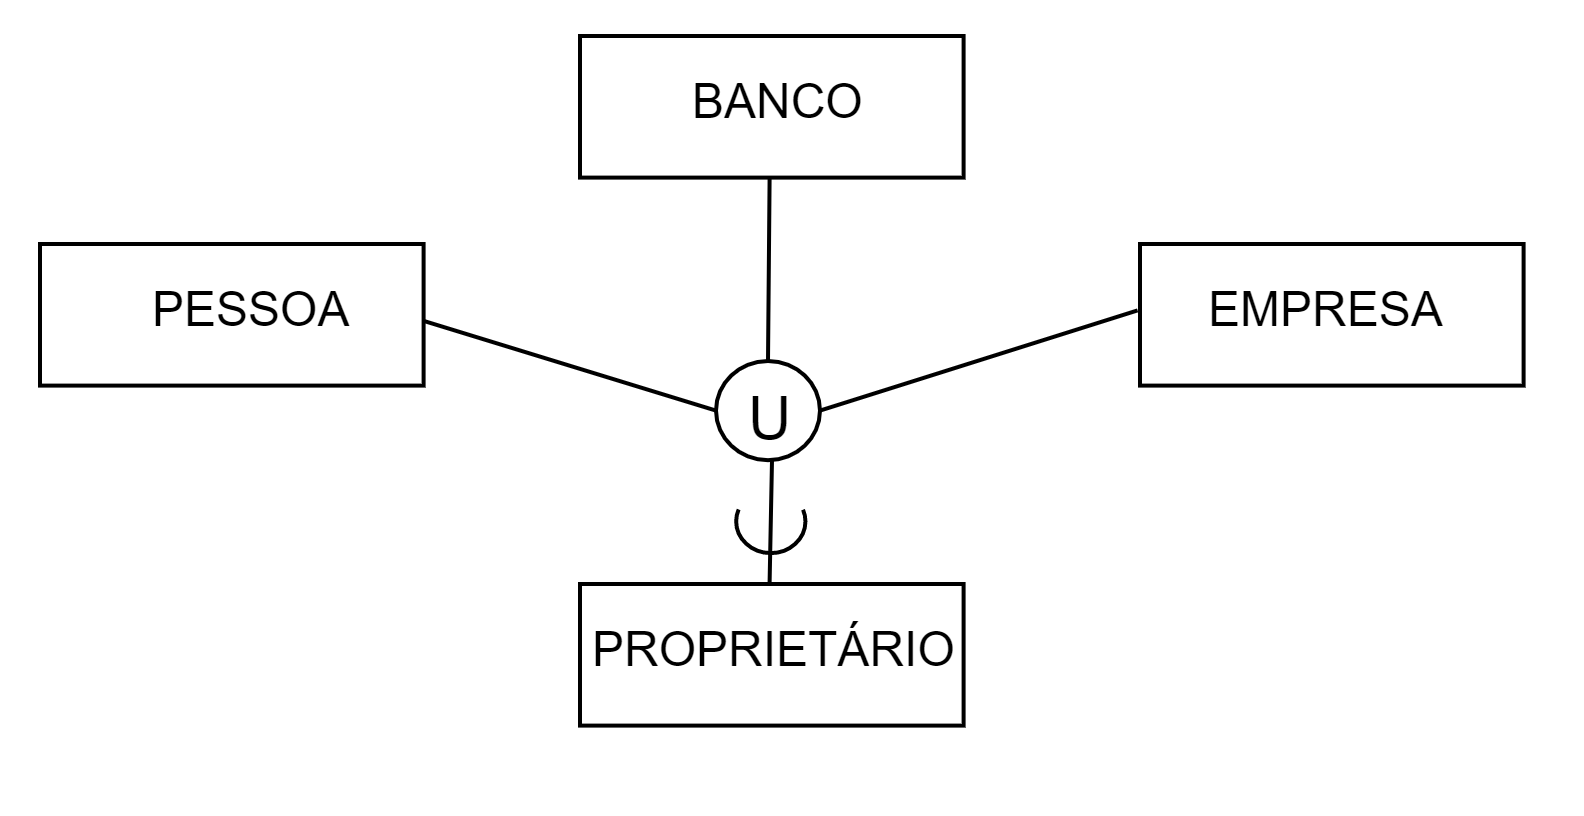
\includegraphics[scale=0.13]{Figuras/02_04.png}
\end{figure}
\end{ftst}

%==================================

\begin{ftst}{Modelagem dos tipos UNIÃO usando categorias}{Modelo Entidade-Relacionamento Estendido}
\begin{figure}
    \centering
    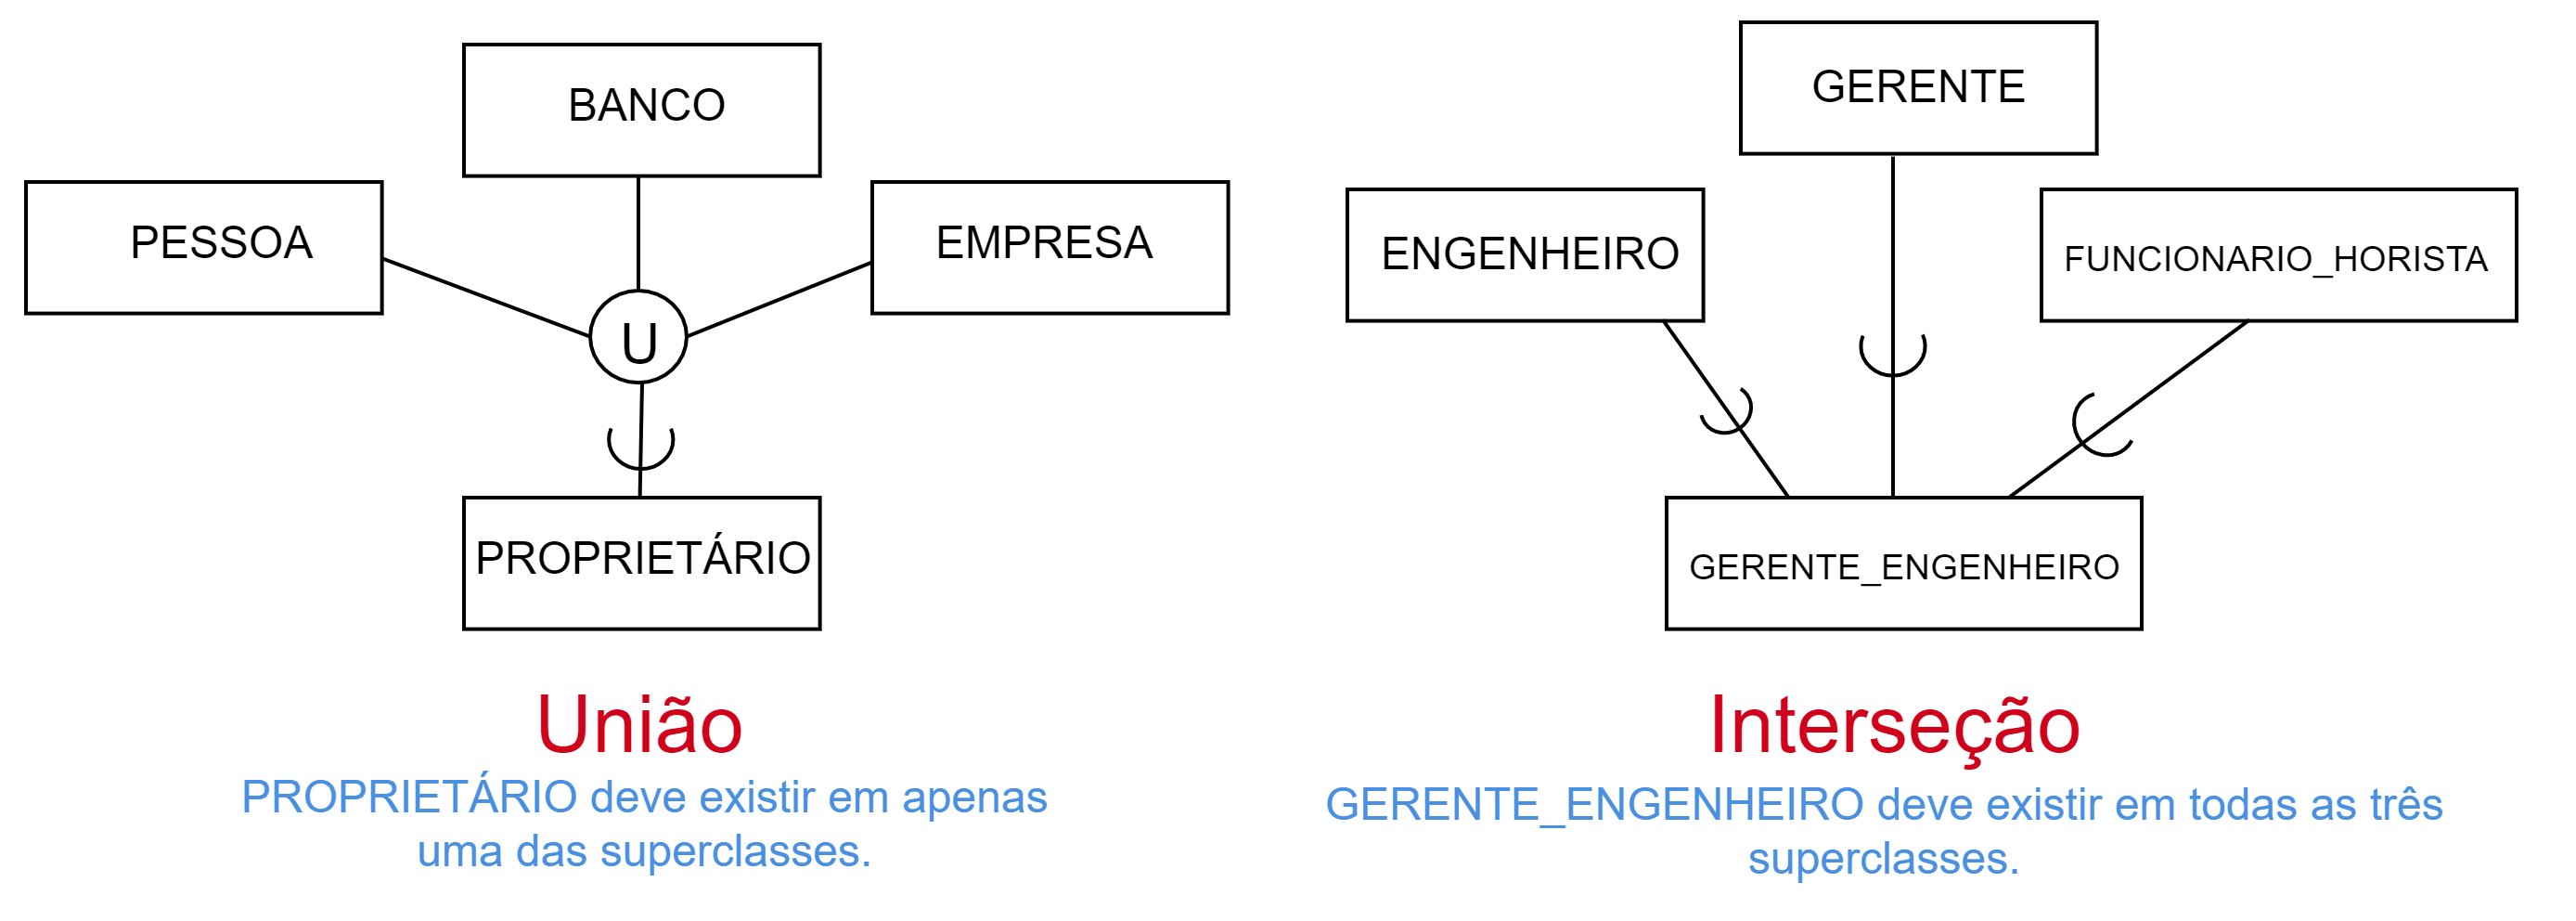
\includegraphics[scale=0.12]{Figuras/02_05.png}
\end{figure}
\footnotesize
\begin{itemize}
    \item A herança de atributo funciona de maneira mais seletiva no caso de categorias. 
    \item Exemplo: PROPRIETÁRIO herda os atributos de uma EMPRESA, uma PESSOA ou um BANCO, dependendo da superclasse à qual a entidade pertence. Já GERENTE\_ENGENHEIRO, herda todos os atributos de suas superclasses FUNCIONARIO\_MENSAL, ENGENHEIRO e GERENTE.
\end{itemize}
\end{ftst}

%==================================

\begin{ftst}{Modelagem dos tipos UNIÃO usando categorias}{Modelo Entidade-Relacionamento Estendido}
\begin{itemize}
    \item Uma categoria pode ser \textbf{total} ou \textbf{parcial}. 
    \item Uma \textbf{categoria total} mantém a união de todas as entidades em suas superclasses, enquanto a \textbf{parcial} pode manter um subconjunto da união. 
    \item Notação: uma categoria total é representada em diagrama por uma linha dupla que conecta a categoria e o círculo, ao passo que uma categoria parcial é indicada por uma linha simples.
    \item Se uma categoria é total (não parcial), ela pode ser
    representada alternativamente como uma especialização total.
    \item Se as duas classes representam o mesmo tipo de entidades e compartilham diversos atributos, incluindo os mesmos atributos-chave, a especialização/generalização é preferida. Caso contrário, a categorização (tipo de união) é mais apropriada.

\end{itemize}
\end{ftst}

%==================================

\begin{ftst}{Modelagem dos tipos UNIÃO usando categorias}{Modelo Entidade-Relacionamento Estendido}
\vone
\begin{figure}
    \centering
    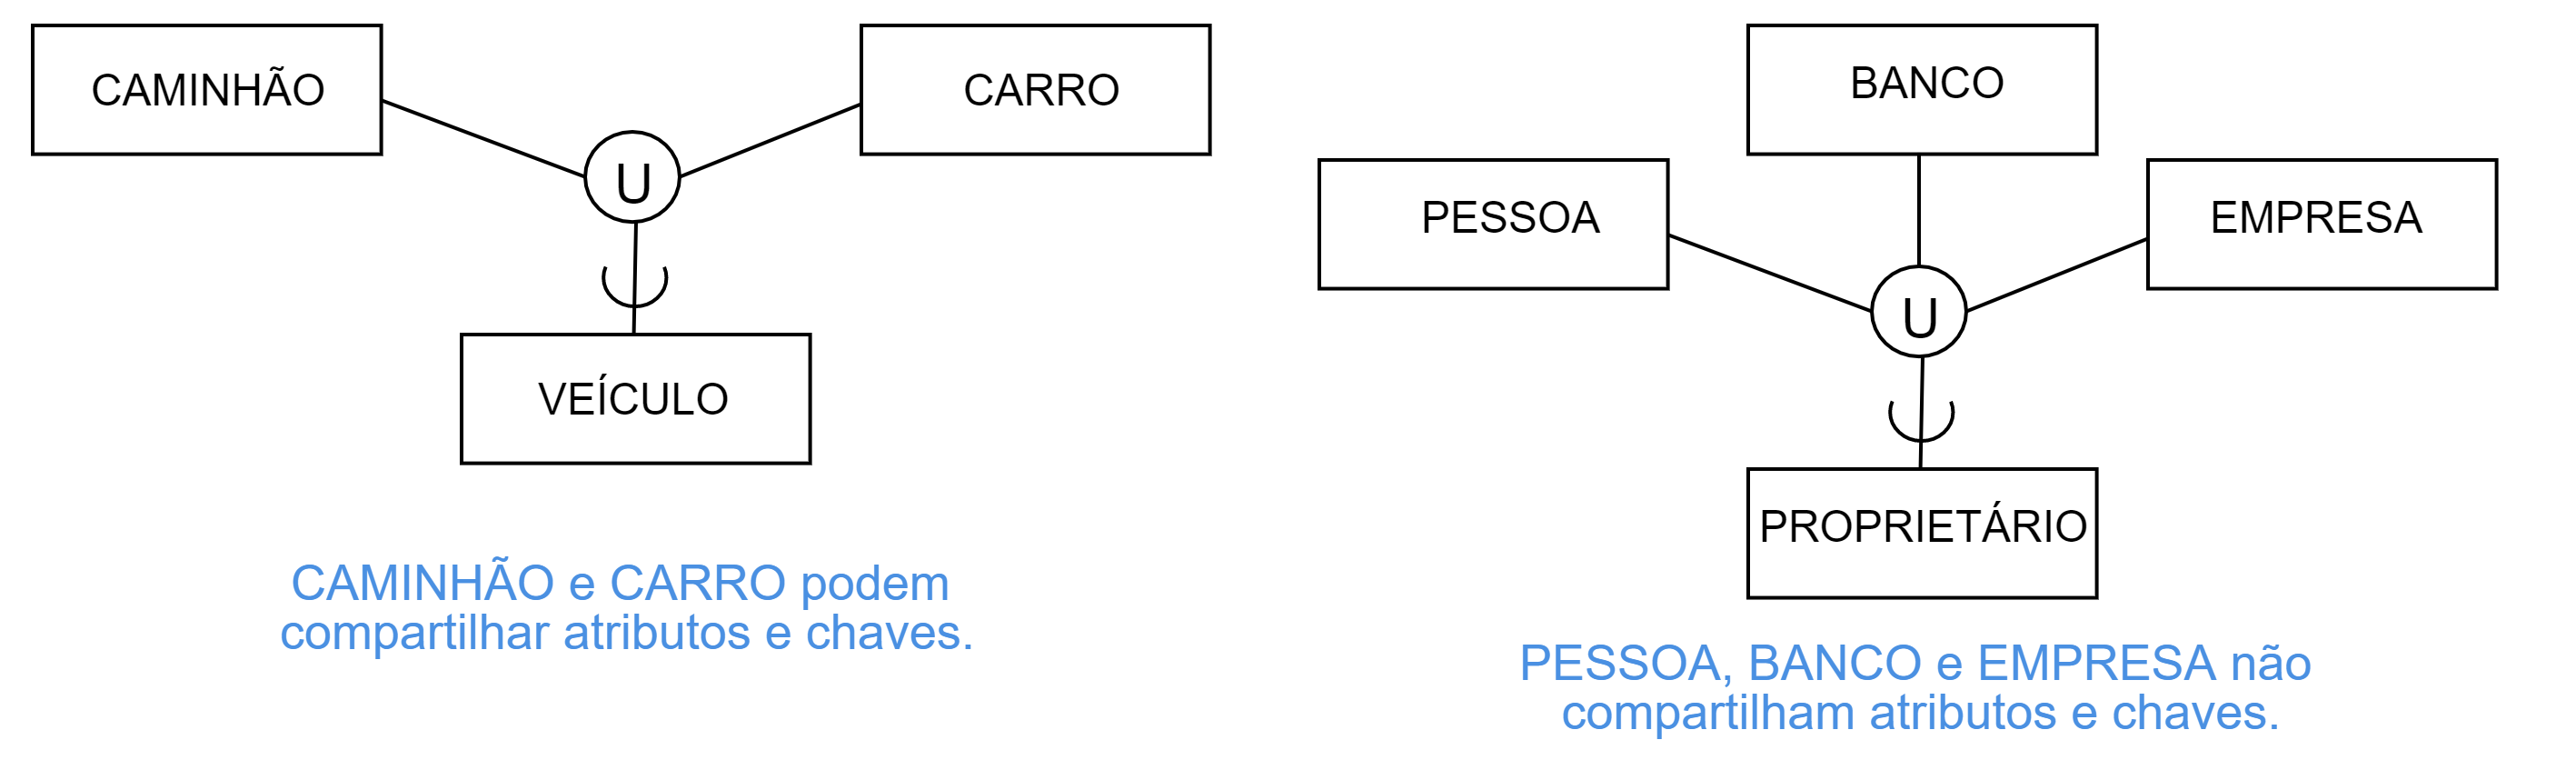
\includegraphics[scale=0.12]{Figuras/02_06.png}
\end{figure}

\end{ftst}


\end{document}